\section{1174006 - Kadek Diva Krishna Murti}

\subsection{Teori}
\begin{enumerate}
	\item Jelaskan dengan ilustrasi gambar sendiri apa perbedaan antara vanilla GAN dan cGAN.\\
    Vanilla GAN merupakan tipe GAN yang paling sederhana. Ia memiliki dua network diantaranya generator network dan discriminator network. Kedua network tersebut akan dilatih dan diadu satu sama lain. Generator network dilatih untuk membodohi discriminator network dengan membuat data baru dari data asli. Discriminator dilatih untuk tidak dibodohi oleh generator network
    \begin{figure}[H]
		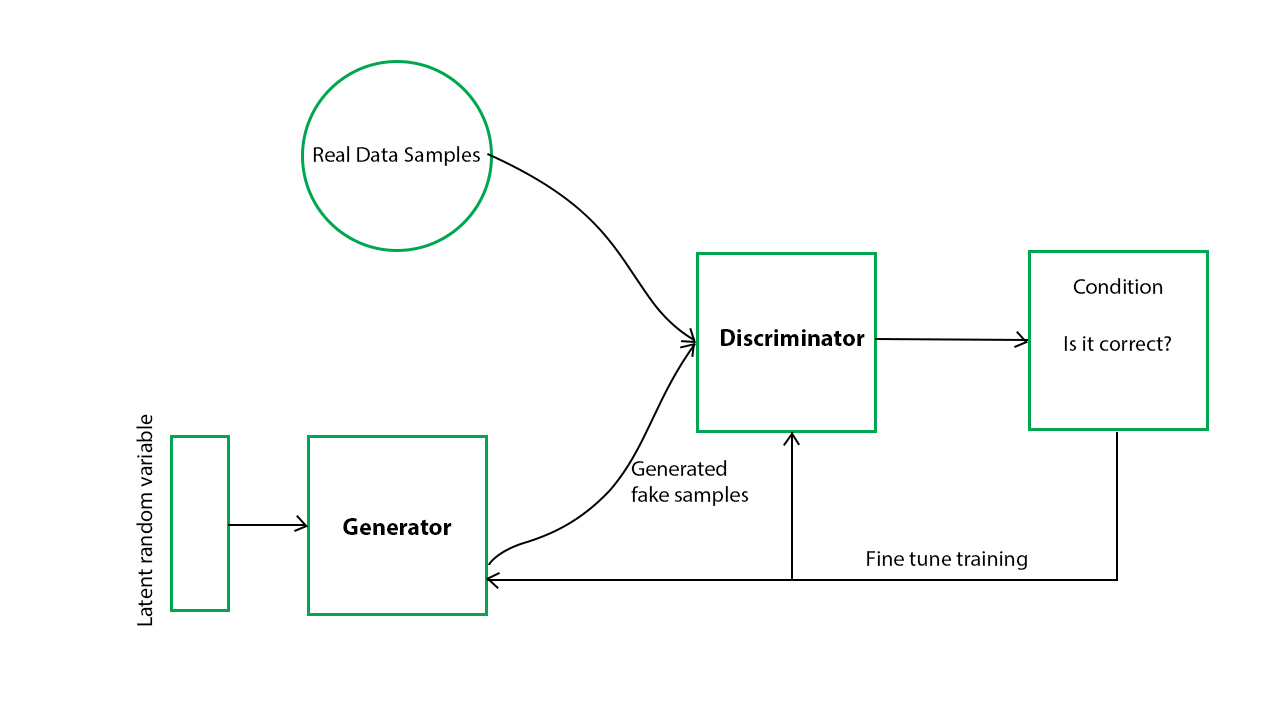
\includegraphics[width=8cm]{figures/1174006/chapter9/teori/vanilla.jpg}
		\centering
    \end{figure}
    CGAN merupakan tipe GAN yang menerapkan metode deep learning dimana memiliki beberapa parameter kondisional pada generator dan discriminator. Parameter tersebut bisa berupa informasi label untuk membantu membedakan data asli dan data palsu.
    \begin{figure}[H]
		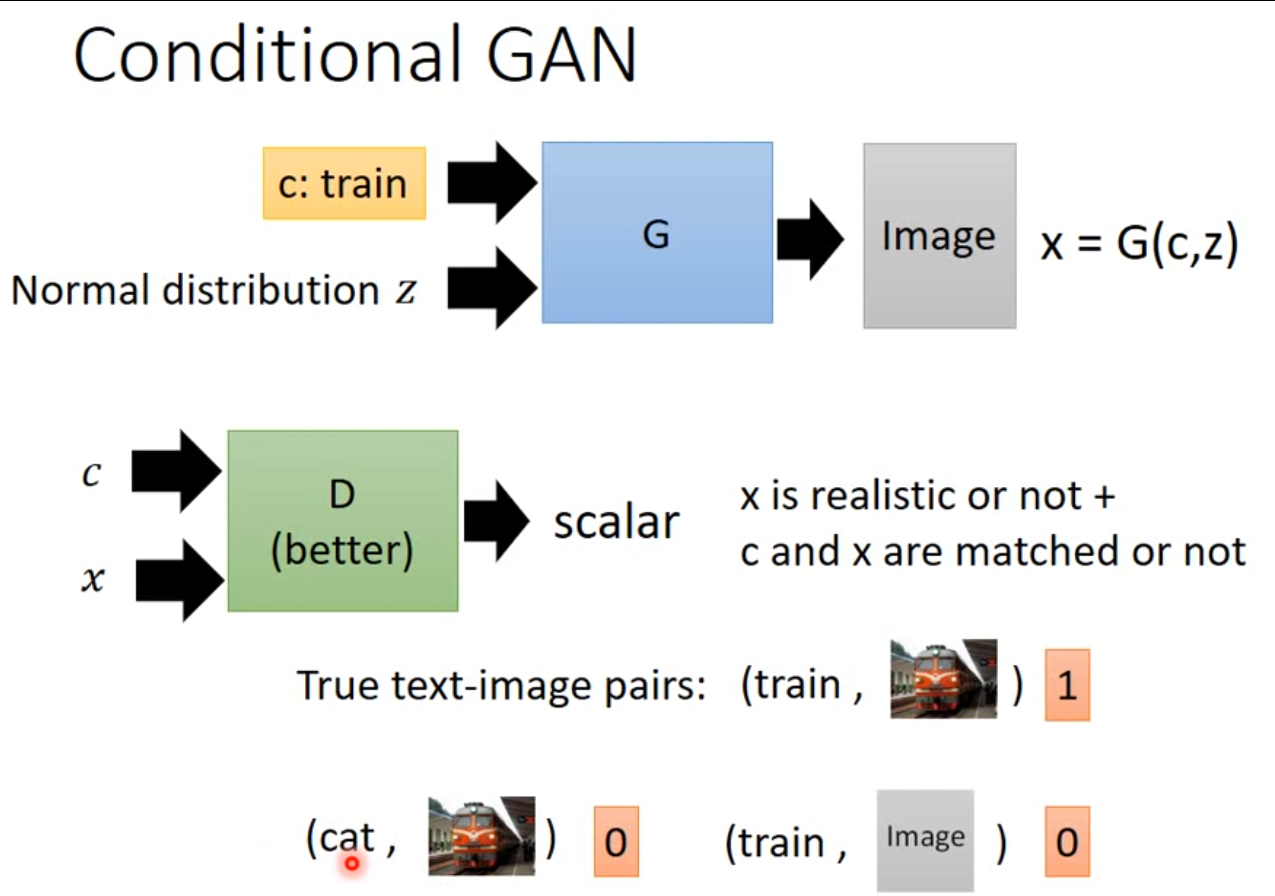
\includegraphics[width=8cm]{figures/1174006/chapter9/teori/cgan.png}
		\centering
	\end{figure}
	\item Jelaskan dengan ilustrasi gambar sendiri arsitektur dari Age-cGAN.\\
    Age-cGAN terdiri dari empat network, diantaranya:
    \begin{itemize}
        \item Encoder, network ini memetakan data input ke dalam bentuk latent vector.
        \item FaceNet, network ini belajar mengenali perbedaan antara data input dengan data hasil generate
        \item Generator Network, network ini mengenerate data baru dari inputan yang ada.
        \item Discriminator Network, network ini mencoba membedakan antara data asli dan data palsu.
    \end{itemize}
	\begin{figure}[H]
		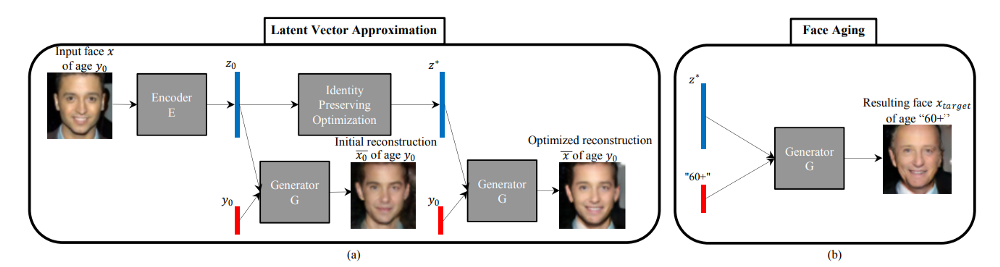
\includegraphics[width=8cm]{figures/1174006/chapter9/teori/agecgan.png}
		\centering
	\end{figure}
    \item Jelaskan dengan ilustrasi gambar sendiri arsitektur encoder network dari AgecGAN.\\
    Encoder network memetakan data input ke dalam bentuk latent vector.
    \item Jelaskan dengan ilustrasi gambar sendiri arsitektur generator network dari AgecGAN.\\
    Generator network mengenerate data baru dari inputan yang ada.
    \item Jelaskan dengan ilustrasi gambar sendiri arsitektur discriminator network dari Age-cGAN.\\
    Discriminator network mencoba membedakan antara data asli dan data palsu.
    \item Jelaskan dengan ilustrasi gambar apa itu pretrained Inception-ResNet-2 Model.
    Pretrained Inception-ResNet-2 Model adalah sebuah model terlatih berdasar jutaan gambar dari ImageNet
    \item Jelaskan dengan ilustrasi gambar sendiri arsitektur Face recognition network Age-cGAN.
    \begin{itemize}
        \item Encoder, network ini memetakan data input ke dalam bentuk latent vector.
        \item FaceNet, network ini belajar mengenali perbedaan antara data input dengan data hasil generate
        \item Generator Network, network ini mengenerate data baru dari inputan yang ada.
        \item Discriminator Network, network ini mencoba membedakan antara data asli dan data palsu.
    \end{itemize}
	\begin{figure}[H]
		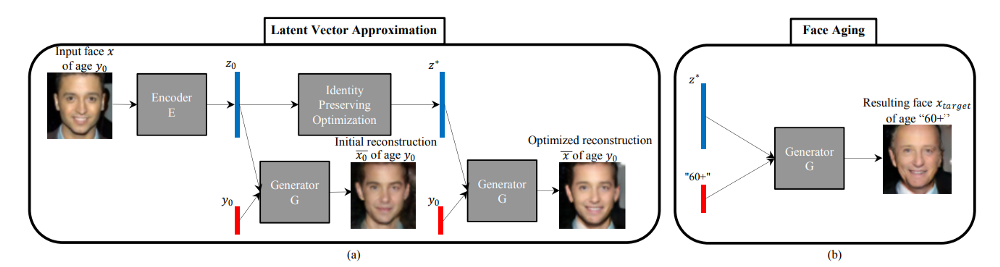
\includegraphics[width=8cm]{figures/1174006/chapter9/teori/agecgan.png}
		\centering
	\end{figure}
    \item Sebutkan dan jelaskan serta di sertai contoh-contoh tahapan dari Age-cGAN
    \begin{itemize}
        \item Encoder, network ini memetakan data input ke dalam bentuk latent vector.
        \item FaceNet, network ini belajar mengenali perbedaan antara data input dengan data hasil generate
        \item Generator Network, network ini mengenerate data baru dari inputan yang ada.
        \item Discriminator Network, network ini mencoba membedakan antara data asli dan data palsu.
    \end{itemize}
	\begin{figure}[H]
		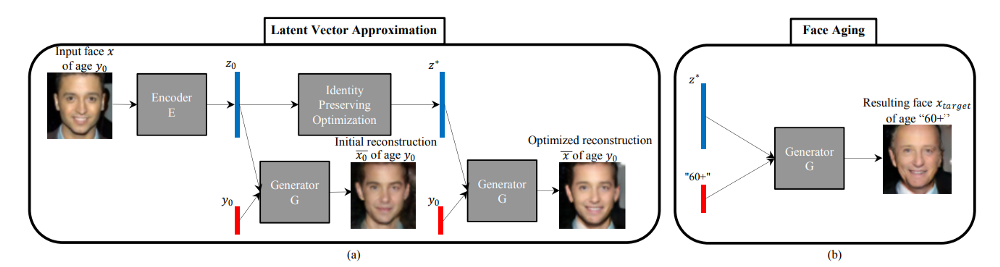
\includegraphics[width=8cm]{figures/1174006/chapter9/teori/agecgan.png}
		\centering
	\end{figure}

    \item Berikan contoh perhitungan fungsi training objektif\\
    Rumus yang dipakai untuk menerapkan fungsi training objektif adalah sebagai berikut:
    \begin{figure}[H]
		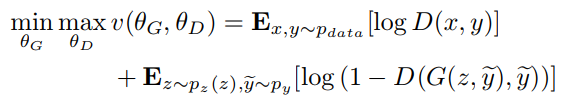
\includegraphics[width=8cm]{figures/1174006/chapter9/teori/tof.png}
		\centering
    \end{figure}
    Penjelasan:\\
    \begin{itemize}
        \item log D (x, y) adalah kerugian pada model Diskriminator.
        \item log (1-D (G (x, y ’), y’)) adalah kerugian pada model Generator.
        \item P (data) adalah distribusi dari semua gambar yang memungkinkan.
    \end{itemize}

    \item Berikan contoh dengan ilustrasi penjelasan dari Initial latent vector approximation
    \begin{itemize}
        \item Initial latent vector approximation merupakan metode yang digunakan untuk memperkirakan vektor latent untuk mengoptimalkan rekronstruksi gambar wajah.
        \item Encoder adalah jaringan saraf yang mendekati vektor latent.
        \item Encoder network dilatih pada gambar yang dihasilkan dan pada gambar asli.
        \item Setelah dilatih, jaringan encoder akan mulai menghasilkan vektor laten dari distribusi yang dipelajari.
        \item Fungsi objektif pelatihan dari pelatihan jaringan network adalah Euclidean distance loss.
    \end{itemize}

    \item Berikan contoh perhitungan latent vector optimization\\
    Latent vector optimization merupakan proses untuk meningkatakan kinerja dari encoder dan generator network secara sekaligus. Rumus yang dipakai untuk menerapkan latent vector optimization adalah sebagai berikut:\\
    \begin{figure}[H]
		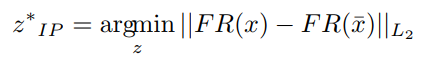
\includegraphics[width=8cm]{figures/1174006/chapter9/teori/lvo.png}
		\centering
	\end{figure}
    Penjelasan:
    \begin{itemize}
        \item FR adalah face recognition network untuk mengenali identitas orang berdasar inputan gambar wajah
        \item Persamaan jarak Euclidean antara gambar asli dan gambar rekrontruksi
        \item Meminimalkan jarak Euclidean ini harus meningkatkan pemeliharaan identitas pada rekronstruksi gambar
    \end{itemize}
\end{enumerate}

\subsection{Praktek}
\begin{enumerate}
	\item Jelaskan bagaimana cara ekstrak file dataset Age-cGAN menggunakan google colab
    \begin{lstlisting}
        !tar -xvf  'wiki_crop.tar' -C './data'
    \end{lstlisting}
    \begin{figure}[H]
		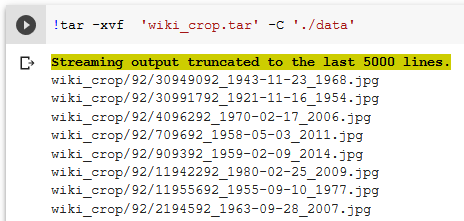
\includegraphics[width=8cm]{figures/1174006/chapter9/praktek/1.png}
		\centering
	\end{figure}
    \item Jelaskan bagaimana kode program bekerja untuk melakukan load terhadap dataset yang sudah di ekstrak, termasuk bagaimana penjelasan kode program perhitungan usia\\
    Cara load dataset, adalah sebagai berikut:
    \begin{lstlisting}
        def load_data(wiki_dir, dataset='wiki'):
            # Load the wiki.mat file
            meta = loadmat(os.path.join(wiki_dir, "{}.mat".format(dataset)))

            # Load the list of all files
            full_path = meta[dataset][0, 0]["full_path"][0]

            # List of Matlab serial date numbers
            dob = meta[dataset][0, 0]["dob"][0]

            # List of years when photo was taken
            photo_taken = meta[dataset][0, 0]["photo_taken"][0]  # year

            # Calculate age for all dobs
            age = [calculate_age(photo_taken[i], dob[i]) for i in range(len(dob))]

            # Create a list of tuples containing a pair of an image path and age
            images = []
            age_list = []
            for index, image_path in enumerate(full_path):
                images.append(image_path[0])
                age_list.append(age[index])

            # Return a list of all images and respective age
            return images, age_list
    \end{lstlisting}
    Penjelasan kode program perhitungan usia, adalah sebagai berikut:
    \begin{lstlisting}
        def calculate_age(taken, dob):
            birth = datetime.fromordinal(max(int(dob) - 366, 1))

            if birth.month < 7:
                return taken - birth.year
            else:
                return taken - birth.year - 1
    \end{lstlisting}
    \item Jelaskan bagaimana kode program The Encoder Network bekerja dijelaskan dengan bahawa awam dengan ilustrasi sederhana
    \begin{lstlisting}
        def build_encoder():
            """
            Encoder Network
            """
            input_layer = Input(shape=(64, 64, 3))
        
            # 1st Convolutional Block
            enc = Conv2D(filters=32, kernel_size=5, strides=2, padding='same')(input_layer)
            # enc = BatchNormalization()(enc)
            enc = LeakyReLU(alpha=0.2)(enc)
        
            # 2nd Convolutional Block
            enc = Conv2D(filters=64, kernel_size=5, strides=2, padding='same')(enc)
            enc = BatchNormalization()(enc)
            enc = LeakyReLU(alpha=0.2)(enc)
        
            # 3rd Convolutional Block
            enc = Conv2D(filters=128, kernel_size=5, strides=2, padding='same')(enc)
            enc = BatchNormalization()(enc)
            enc = LeakyReLU(alpha=0.2)(enc)
        
            # 4th Convolutional Block
            enc = Conv2D(filters=256, kernel_size=5, strides=2, padding='same')(enc)
            enc = BatchNormalization()(enc)
            enc = LeakyReLU(alpha=0.2)(enc)
        
            # Flatten layer
            enc = Flatten()(enc)
        
            # 1st Fully Connected Layer
            enc = Dense(4096)(enc)
            enc = BatchNormalization()(enc)
            enc = LeakyReLU(alpha=0.2)(enc)
        
            # Second Fully Connected Layer
            enc = Dense(100)(enc)
        
            # Create a model
            model = Model(inputs=[input_layer], outputs=[enc])
            return model
    \end{lstlisting}
    Encoder, network ini memetakan data input ke dalam bentuk latent vector.
    \item Jelaskan bagaimana kode program The Generator Network bekerja dijelaskan dengan bahawa awam dengan ilustrasi sederhana
    \begin{lstlisting}
        def build_generator():
            """
            Create a Generator Model with hyperparameters values defined as follows
            """
            latent_dims = 100
            num_classes = 6

            input_z_noise = Input(shape=(latent_dims,))
            input_label = Input(shape=(num_classes,))

            x = concatenate([input_z_noise, input_label])

            x = Dense(2048, input_dim=latent_dims + num_classes)(x)
            x = LeakyReLU(alpha=0.2)(x)
            x = Dropout(0.2)(x)

            x = Dense(256 * 8 * 8)(x)
            x = BatchNormalization()(x)
            x = LeakyReLU(alpha=0.2)(x)
            x = Dropout(0.2)(x)

            x = Reshape((8, 8, 256))(x)

            x = UpSampling2D(size=(2, 2))(x)
            x = Conv2D(filters=128, kernel_size=5, padding='same')(x)
            x = BatchNormalization(momentum=0.8)(x)
            x = LeakyReLU(alpha=0.2)(x)

            x = UpSampling2D(size=(2, 2))(x)
            x = Conv2D(filters=64, kernel_size=5, padding='same')(x)
            x = BatchNormalization(momentum=0.8)(x)
            x = LeakyReLU(alpha=0.2)(x)

            x = UpSampling2D(size=(2, 2))(x)
            x = Conv2D(filters=3, kernel_size=5, padding='same')(x)
            x = Activation('tanh')(x)

            model = Model(inputs=[input_z_noise, input_label], outputs=[x])
            return model
    \end{lstlisting}
    Generator Network, network ini mengenerate data baru dari inputan yang ada.
    \item Jelaskan bagaimana kode program The Discriminator Network bekerja dijelaskan dengan bahawa awam dengan ilustrasi sederhana
    \begin{lstlisting}
        def build_discriminator():
            """
            Create a Discriminator Model with hyperparameters values defined as follows
            """
            input_shape = (64, 64, 3)
            label_shape = (6,)
            image_input = Input(shape=input_shape)
            label_input = Input(shape=label_shape)

            x = Conv2D(64, kernel_size=3, strides=2, padding='same')(image_input)
            x = LeakyReLU(alpha=0.2)(x)

            label_input1 = Lambda(expand_label_input)(label_input)
            x = concatenate([x, label_input1], axis=3)

            x = Conv2D(128, kernel_size=3, strides=2, padding='same')(x)
            x = BatchNormalization()(x)
            x = LeakyReLU(alpha=0.2)(x)

            x = Conv2D(256, kernel_size=3, strides=2, padding='same')(x)
            x = BatchNormalization()(x)
            x = LeakyReLU(alpha=0.2)(x)

            x = Conv2D(512, kernel_size=3, strides=2, padding='same')(x)
            x = BatchNormalization()(x)
            x = LeakyReLU(alpha=0.2)(x)

            x = Flatten()(x)
            x = Dense(1, activation='sigmoid')(x)

            model = Model(inputs=[image_input, label_input], outputs=[x])
            return model
    \end{lstlisting}
    Discriminator Network, network ini mencoba membedakan antara data asli dan data palsu.
    \item Jelaskan bagaimana kode program Training cGAN bekerja dijelaskan dengan bahawa awam dengan ilustrasi sederhana
    Cara kerja program Training cGAN, adalah sebagai berikut:
    \begin{itemize}
        \item Gambar asli yang akan diproses.
        \item Rekronstruksi gambar yang telah digenerate menggunakan initial latent approximations z0.
        \item Rekronstruksi gambar yang telah digenerate menggunakan "Pixelwise" and "Identity-Preserving" lalu dilakukan optimasi menggunakan latent approximations: z ∗ pixel and z ∗ IP.
        \item penentuan umur berdasar gambar generate yang telah direkrontruksi menggunakan identity-preserving z ∗ IP latent approximations and kondisi dari berbagai label umur y (one per column).
    \end{itemize}
	\begin{figure}[H]
		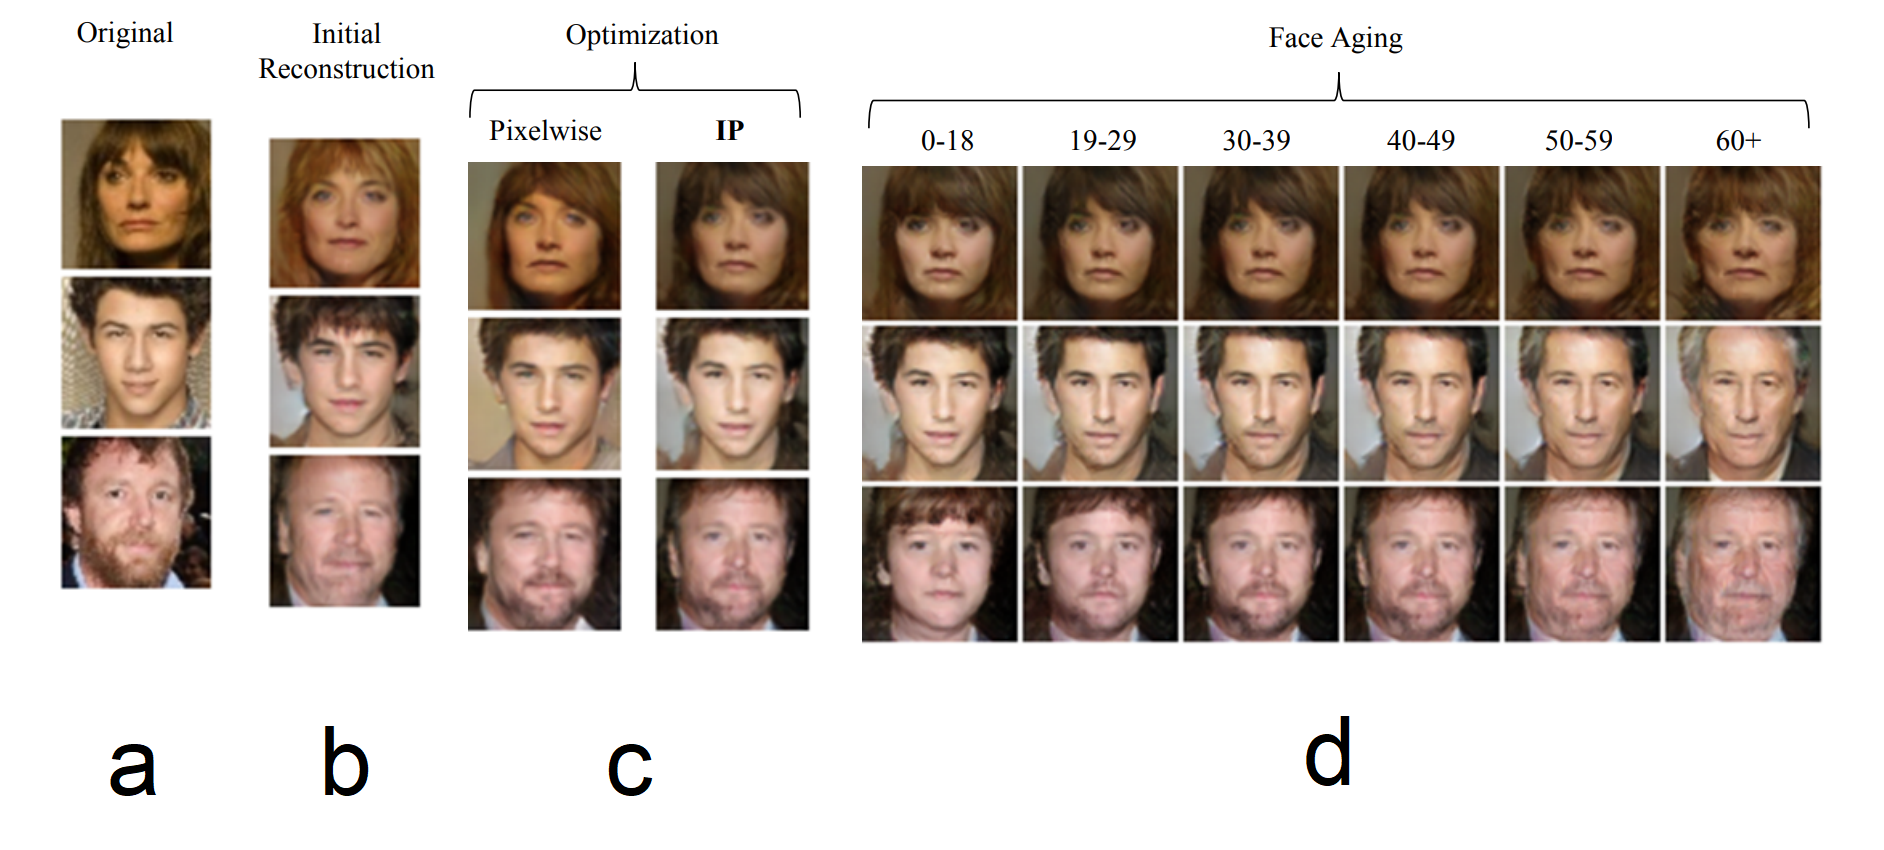
\includegraphics[width=8cm]{figures/1174006/chapter9/praktek/proses.png}
		\centering
	\end{figure}
    \item Jelaskan bagaimana kode program Initial dan latent vector approximation bekerja dijelaskan dengan bahawa awam dengan ilustrasi sederhana
    \begin{itemize}
        \item Initial latent vector approximation merupakan metode yang digunakan untuk memperkirakan vektor latent untuk mengoptimalkan rekronstruksi gambar wajah.
        \item Encoder adalah jaringan saraf yang mendekati vektor latent.
        \item Encoder network dilatih pada gambar yang dihasilkan dan pada gambar asli.
        \item Setelah dilatih, jaringan encoder akan mulai menghasilkan vektor laten dari distribusi yang dipelajari.
        \item Fungsi objektif pelatihan dari pelatihan jaringan network adalah Euclidean distance loss.
    \end{itemize}
\end{enumerate}

\subsection{Penanganan Error}
\begin{enumerate}
	\item Skrinsut error
    \item Tuliskan kode eror dan jenis errornya
    \item Solusi pemecahan masalah error tersebut
\end{enumerate}